\documentclass[]{article}
\usepackage{biblatex}
\usepackage{graphicx}
\usepackage{float}
\usepackage{listings}
\usepackage{selinput}
\usepackage{amsmath}

\addbibresource{bib.bib}

\title{Optical Flow with Convolutional Neural Networks}
\author{Sean Batzel\\Subhashini Arunachalam\\Shyam Senthil Nathan}

\begin{document}

\maketitle
\nocite{*}

\begin{abstract}
    Optical flow analysis is the estimation of the relative positions or apparent motion of objects in subsequent image frames.
    There are a few methods of estimation of optical flow in use.
    The paper that our work is based on uses the Lucas-Kanade method to calculate optical flow and models convolutional neural networks based on the results, with the goal of introducing a procedure for fine-tuning of the convolutional neural networks for optical flow estimation.
    In this work, we shall demonstrate improvements to the original paper’s standing process for processing optical flow with a convolutional neural network by employing the pyramidal approach to the Lucas-Kanade method.
    We shall implement mini-batch gradient descent over the established stochastic gradient descent to further optimize the learning function employed by the paper and determine the process’ capacity to be trained by an animated scenario, rather than purely by real-life footage.
    We shall finally test the performance and behavior benefits of an eigenvalue-based approach to the Lucas-Kanade method of optical flow tracking over the least squares method.
    We hope to gain considerable improvements to performance with our modifications.
\end{abstract}

\section{Introduction}\label{sec:introduction}
Optical flow estimation plays an important role in many of the modern computer vision applications such as self-driving cars and augmented reality games and applications. 
There are a few prominent methods of estimation of optical flow such as phase correlation, Lucas-Kanade method, Horn-Schunck method, and Buxton-Buxton method. Of these, The Lucas-Kanade method is one of the more widely used and well-performing methods, and is in use across various applications. 
While all these methods are strictly rooted in straight-forward mathematical algorithms, there has been little work done in the estimation of optical flow using AI models, more specifically, convolutional neural networks. 
Convolutional neural networks are a class of deep neural networks that is commonly use in analyzing images. 
Convolutional neural networks can be less resource-intensive than traditional mathematical algorithms in estimating optical flow, and hence can be a good fit to model and determine optical flow estimations between images.

Our work is based on Flett's \textit{The Implementation of Optical Flow in Neural Network} which looks at this approach of estimating optical flow \cite{flett}. 
The paper has a number of areas of improvement that have been identified, and we have implemented a few of those improvements in our work, with the overall goal of advancing the estimation of optical flow using neural networks.\footnote{In general, this work should be considered as a series of patches to Flett's work, as the same methods as outlined in the paper will be used in the construction of the neural network, deviating as little as possible so as to maintain the integrity of the original work.
All code adapted from Flett's work has been cited as such.}

\section{Related Work}\label{sec:related-work}
Flett has designed a convolutional neural network that is modeled on optical flow estimations from the Lucas-Kanade method. 
The convolutional network is then tested with new inputs and its performance has been measured and compared with the traditional methods, and over various versions. 
There are a few shortcomings to this work that we have identified, and that were identified in the original work. 
Flett's implementation is based on results from the Lucas-Kanade method which works best only for very small motion in images, to the tune of around 1 pixel in dimensions. 
This can be a restricting factor to testing and working with images with relatively larger motions between them. 
The original implementation used the least-squares method to calculate optical flow in the Lucas-Kanade method. 
While the results of this method are on par with using the eigenvalues approach, there is a performance disadvantage to using the least squares method.
In the convolutional neural networks, Flett's implementation used the stochastic gradient descent method in modeling the networks, while there are better methods available for the purpose. 
Lastly, part of Flett's implementation is in MATLAB, which is proprietary software, which may undermine the ability of researchers and engineers to adapt this implementation for their needs.\cite{flett}

FlowNet: Learning Optical Flow With Convolutional Networks \cite{fischer} implements a convolutional neural network that models optical flow estimation as a supervised learning task and achieves commendable results.  
Optical Flow Estimation in the Deep Learning Age \cite{roth} takes a look at some of the existing implementations of optical flow estimations that use deep and convolutional neural networks, and presents a story of how the field has evolved. It also compares the various approaches, and identifies the most promising and seminal works. 
How Do Neural Networks Estimate Optical Flow? A Neuropsychology-Inspired Study \cite{jong} looks at how neural networks that model optical flow work by delving deep into the working of the CNN that they created, and providing a comparison with a biological brain's processing of the same data. 

\section{Goals}\label{sec:goals}
The improvements and changes that we set out to make to the original paper by Flett are as follows:

\begin{itemize}
  \item To implement the pyramidal Lucas-Kanade method as opposed to the single-level Lucas-Kanade method in the original paper to overcome its limitation of being able to detect flow accurately only for very small amounts of motion, to the tune of a single pixel.
  
  \item To use the eigenvalues approach to calculate the displacements in the Lucas-Kanade method, as opposed to the least squares method used, to gain improvements in terms of efficiency.
  
  \item To use the mini-batch gradient descent method instead of the stochastic gradient descent method in the convolutional neural networks to determine if it can provide better results than the original
  
  \item To implement the whole project using open-source technologies, eliminating the usage of MATLAB in the original paper, to better aid researchers and  engineers looking to adapt this work\footnote{This was done by adapting source code modified from our collective solutions to the Lucas-Kanade implementation, in order to avoid reinventing the wheel.}
  
  \item To test the convolutional neural network by training it with animated (cartoon) images and determining if there is any significant changes in the performance of the CNN
\end{itemize}

\section{Implementation}\label{sec:implementation}
We have taken the original implementation by Flett, the code for which was available in the paper, and have made our modifications and improvements and modifications to it. The artifacts of our work can be found at \url{https://github.com/Romulus10/CS583-Final-Project}. 

\subsection{Pyramidal Lucas-Kanade}\label{subsec:pyramidal-lucas-kanade}
Pyramidal execution of the classical Lucas-Kanade algorithm is used to deal with large pixel flows for small window of integration and to get higher accuracy.
An image is represented in the form of a pyramid. If an image $I$ has width $n_x$ and height $n_y$, then pyramidal form of that image is obtained in a recursive manner: $I^1$ from $I^0$, $I^2$ from $I^1$ and so on.
Given a point $u$ in the first frame/image, the corresponding location $v=u+d$ in the second frame/image is tracked, where $d$ is the displacement vector.
When two images along with initial displacement is provided as input, pyramidal forms the images are built and updated displacement is computed at each level using iterative optical flow computation.
We used multiple images with motion flows between them and calculated optical flow for our data-set using the pyramidal Lucas-Kanade method, and used the results from this to train the convolutional neural network \cite{bouguet}.

\subsection{Mini-batch Gradient Descent}\label{subsec:mini-batch-gradient-descent}
The cited paper had used stochastic gradient descent optimizer method to train the neural networks and update weights to nodes across the network.
Current state of the model is used to make a prediction and prediction is compared against the expected values to find the error gradient.
Computed error gradient is used to update the weights of the model repeatedly.
In the Stochastic algorithms the batch size is set to 1 and it use only one example at a time.
Since stochastic use only one example at a time, it is not possible to implement the vectorized implementation and it could slow down the computations.
In order to handle this problem, we have used the mini-batch gradient descent in our implementation for which the batch size is set greater than 1 and less than the number of training samples $1 < bs < m$, where bs is the batch size and m is the total number of examples in the training set$)$.
We have used a batch size of 32 in our implementation \cite{brownlee}.

\subsection{Eigenvalue-Based Optical Flow Computation}\label{subsec:eigenvalue-based-optical-flow-computation}
Motion is estimated of each pixel of an image and then motion of entire image is computed.
In order to address the problem when we have more equations than unknowns, we used least squares method to address it.
Equation could be represented as follows
\begin{center} $(A^T A) d = A^T b$ \end{center}
\setlength{\parskip}{10pt plus 1pt minus 1pt}
where  $ A^T A  =  \begin{bmatrix}
                    \Sigma I_xI_x  & \Sigma I_xI_y    \\
                    \Sigma I_xI_y  & \Sigma I_yI_y 
                    \end{bmatrix} $  and $A^T b = \begin{bmatrix}
                                                   \Sigma I_xI_t  \\
                                                   \Sigma I_yI_t
                                                   \end{bmatrix}$
\setlength{\parskip}{10pt plus 1pt minus 1pt}

In order to solve the above equation, $A^T A$ must be invertible (eigenvalues of $A^T A$ should be $\lambda_1 \geq \lambda_2 > 0$).
To solve for displacement with the above matrices, instead of the least squares approach in the original paper, we have computed eigenvalues of the $A^T A$ matrix, and used them in the calculation of the displacement instead of the matrices themselves.

\subsection{Python Implementation}\label{subsec:python-implementation}
The cited paper's implementation of the Lucas-Kanade optical flow algorithm was originally in MATLAB.
By using the Optical Flow assignment we completed for this course as a starting point, we re-implemented the Lucas-Kanade procedure in pure Python with \texttt{numpy}.
This work is located in \verb|optical_flow.py|.
Since \texttt{numpy} is open source, in contrast to MATLAB, our implementation can be easily adopted by researchers and engineers looking to use this work.

\subsection{Training on Animated Scenes}\label{subsec:training-on-animated-scenes}
This didn't require any changes in the implementation itself.
In testing the training process on animated input, all we needed was to select an animated scene, point out a set of features to track, and feed the optical flow data through the neural network.

\section{Results}\label{sec:result}
This approach to training the neural net produced a marked improvement to the accuracy of the prediction model outlined in \textit{The Implementation of Optical Flow in Neural Networks}.\cite{flett}
Whereas the original model, among all four versions discussed in Flett's paper, reached a peak accuracy of roughly 85\% on 500 epochs of training, ours reached the vicinity of 100\% on the same number of epochs.
We also reached a loss of roughly 1\%, as opposed to the best in the reference material of approximately 25\%.
Our accuracy and loss graphs were as follows:

\begin{figure}[H]
    \centering
    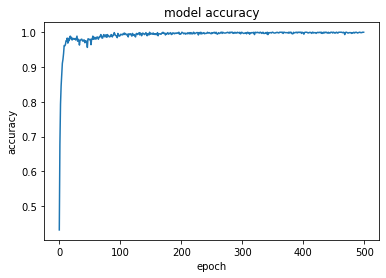
\includegraphics[width=\textwidth]{output_23_0.png}
    \caption{The plot of the determined accuracy per epoch for our prediction model.}
    \label{fig:accuracy}
\end{figure}

\begin{figure}[H]
    \centering
    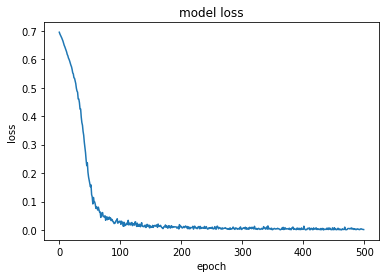
\includegraphics[width=\textwidth]{output_25_0.png}
    \caption{The plot of the determined loss per epoch for our prediction model.}
    \label{fig:loss}
\end{figure}

Also notable is the extremely close correlation between the results of the actual Lucas-Kanade method employed and the bounding box produced by the prediction model:

\begin{figure}[H]
    \centering
    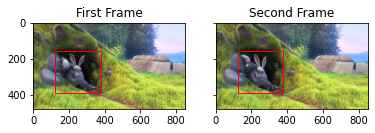
\includegraphics[width=\textwidth]{output_14_0.png}
    \caption{The bounding box translation computed by the strict Lucas-Kanade optical flow algorithm.}
    \label{fig:optical_flow}
\end{figure}

\begin{figure}[H]
    \centering
    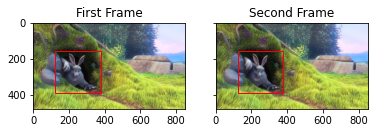
\includegraphics[width=\textwidth]{output_29_0.png}
    \caption{The bounding box translation predicted by our neural network.}
    \label{fig:optical_flow_neural_net}
\end{figure}

\section{Scope for Improvements}\label{sec:improvements}
There are improvements that were suggested in the original paper that we have not implemented, but still apply to our work.
More weight can be added to the central pixels in the frames to allow for images with less edges and structures, such as a plain background, to produce better results from the Lucas-Kanade method.
The eigenvalues can also be used to determine whether certain areas of the image that are being considered as movement are actually just areas of noise and not real movement.
Improvement could also be made to the actual optical flow calculation through the "Good Features to Track" algorithm.\cite{features}

\section{Conclusion}\label{sec:conclusion}
The goal was to train the neural network to a specific algorithm that results in the best performance, in terms of accuracy.
Our usage of the pyramidal Lucas-Kanade method in computing opticalflow, and the mini-batch gradient descent method in the convolutional neural networks, have resulted in vastly improved performance metrics.
This system offers huge scope of improvement and it could prove useful in real-world applications.

\listoffigures

\printbibliography

\end{document}
